\documentclass[]{standalone}
\usepackage{mathptmx}
%\renewcommand{\familydefault}{\rmdefault}
\usepackage[T1]{fontenc}
\usepackage[latin9]{inputenc}
\usepackage{siunitx}
\usepackage{array}
\usepackage{amsmath}
\usepackage{ifthen}
\usepackage{pgfplots}
\pgfplotsset{compat=1.14}
\usepackage{titling, graphicx}
\usepackage{tikz}
\usepackage{upgreek}
\usepackage{amsmath,amsthm}
\usepackage{strtikz}
\usetikzlibrary{shapes,arrows.meta,intersections,graphs,graphs.standard,math,fit}
\usetikzlibrary{calc,intersections,through,backgrounds}
\usetikzlibrary{decorations.pathmorphing, decorations.markings,decorations.pathreplacing}


\begin{document}
\begin{tikzpicture}
\framestructure[%
number of storys=3,
number of bays=2,
story height=1cm,
bay width=2cm,
startX=0cm,
startY=0cm,
line thickness = 1pt,
beam line thickness =1.5pt,
column line thickness = 1.5pt,
foundation side width = 0.75cm,
support width = 0.3cm,
support height = 0.3cm,
support line thickness = 1.0pt,
show supports = 5,
isolator width = 0.4cm,
isolator thickness = 0.2cm,
isolator line thickness = 1.5pt,
foundation thickness = 0.3cm,
mass radius = 2pt,
show mass = 0,
%DOF properties
dof floor = 1,
dof column = 2,
arrow length ratio = 0.4,
dof x rotation = 90,
dof y rotation = -80,
dof r rotation = -30,
rotation dof start angle = 120,
rotation dof end angle = 300,
dof offset ratio = 0.0,
dof xstring = $x$,
dof ystring = $y$,  
dof rstring = $r$,
show dof=0,
show dofx = 0,
show dofy = 0,
show dofr = 1,
show axes=0,
%Pile foundation properties
subfloor number=1,
left soil distance = 1.5cm,
right soil distance = 1.5cm,
left soil depth = 1cm,
right soil depth = 1cm,
soil below foundation = 3cm,
left control distance x = 1.5cm,
left control distance y = 1.5cm,
right control distance x = 1.5cm,
right control distance y = 1.5cm,
axis seperation = 0.2cm,
x axis length = 0.5cm,
y axis length = 0.5cm,
show piles=1,
number of piles=7,
pile depth=2cm,
pile side space=0.5cm,
pile diameter=0.2cm,
pile line thickness=1pt,
show lateral load = 1,
lateral load shift=0.5cm,
lateral load type=0,
top arrow length=1.0cm,
base arrow length=0.75cm,
show deflection = 0,
interstory drift = 0.3cm,
defl parameter x = -0.2cm,
defl parameter y = 0.5cm,
defl parameter base=0.6cm]
\end{tikzpicture}
\end{document}